\section{Background \& Motivation}
\label{sec:Motivation}

\autoref{fig:MT} (left) depicts the various components of (a simplified, unary) MT. 
An input model $\mathsf{M}_{_{\mathsf{in}}}$, conforming to a source metamodel 
$\mathsf{MM}_{_{\mathsf{src}}}$, is transformed into an output model 
$\mathsf{M}_{_{\mathsf{out}}}$, hopefully conforming to a target metamodel
$\mathsf{MM}_{_{\mathsf{tgt}}}$, by the execution of an MT specification.

\begin{figure}[t]%
   \begin{minipage}[t]{0.48\columnwidth}
      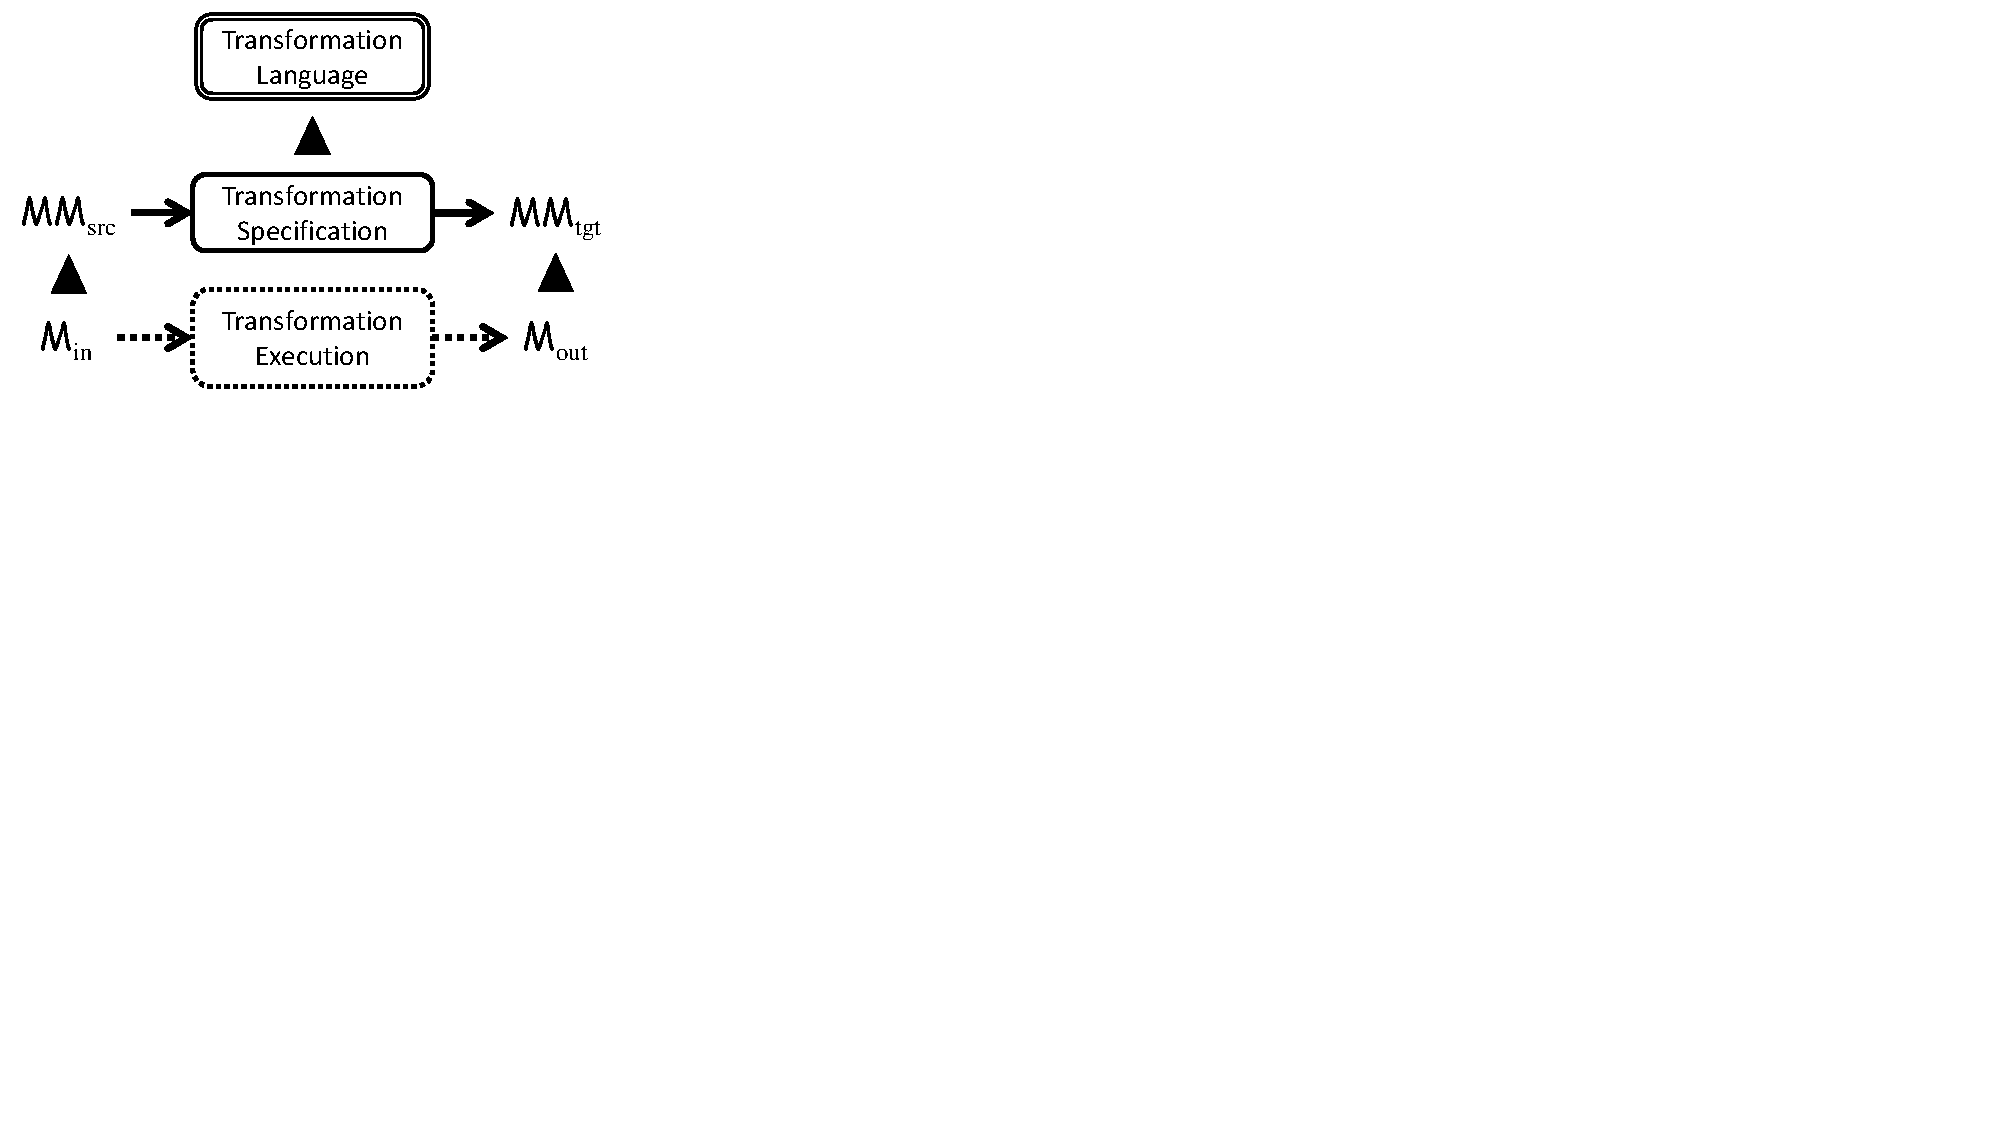
\includegraphics[width=\columnwidth,page=1,clip, trim=0.3cm 12.5cm 23.5cm 0.2cm]{ModelTransformation.pdf}
   \end{minipage}
   \hfill
   \begin{minipage}[b]{0.48\columnwidth}
   \includegraphics[width=\columnwidth,page=2,clip, trim=0.5cm 13.7cm 19.3cm 0cm]{ModelTransformation.pdf}%
   \end{minipage}
   \caption{Model \emph{Transformation} (MT) (left) and Model \emph{Animation} (MA),
   as a special case of MT, operating on the \emph{concrete syntax} of model $\mathsf{M}$,
   which is involved in an endogenous, in-place \emph{simulation} MT. Metamodels
   $\mathsf{MM}$ and $\mathsf{MM}_{\mathsf{CS}}$ may be related through rendering/parsing}%
   \label{fig:MT}%
   \Description[<short description>]{<long description>}
\end{figure}


MTs are not created equal: whereas they may seem syntactically, and sometimes 
semantically, similar, they may serve different purposes (known as MT intents
\citep{J:Lucio-Amrani-etAl:2014} in the literature) that need to be adequately
distinguished. For an input model \textsf{M},
\begin{description}
   \item[Visualisation] is an intent characterising an outplace, heterogeneous
   MT aiming at visually \emph{representing}, or \emph{rendering}, \textsf{M} 
   through the definition of a \emph{visual} concrete syntax based on graphical 
   symbols.
   
   \item[Simulation] is an intent characterising an inplace, endogeneous MT aiming
   at defining \textsf{M}'s operational semantics, i.e. how \textsf{M} evolves 
   over time during when executed.
   
   \item[Animation] is ``\emph{the visual representation of a simulation}'' 
   \citep{J:Lucio-Amrani-etAl:2014}, i.e. it visually renders the computations steps
   defined by the MT simulation specification, by visually projecting the changes
   operated on the simulated model through its (visual) concrete syntax.
\end{description}
Summerising, an \emph{animation} is tightly connected to a \emph{simulation}, and
makes use of a \emph{visualisation}. In other terms, designing an MA requires the
following components, as depicted in \autoref{fig:MT} (right):
\begin{itemize}
	\item A Concrete Syntax \textsf{CS} that should be defined over \textsf{MM}, so
   that it becomes possible to \emph{visualise} \textsf{M} as a graphical model 
   $\mathsf{M}_{\mathsf{CS}}$.
   
   \item \textsf{MM}'s operational semantics is specified in a \emph{simulation}
   MT (specification).
   
   \item \emph{during} each run of the simulation's execution, the computing steps
   are visually rendered over $\mathsf{M}_{\mathsf{CS}}$.
\end{itemize}

Just like MTs are built over transformation \emph{units}, i.e. basic building blocks
that are composed to realise larger, complex transformations, it is likely that 
MA requires a similar decomposition process into basic ``units'' to build and 
organise them. However, MTs are likely specified independently of any MA, primarily
for capturing the \DSL's behaviour, but also likely for supporting other activities
(typically, code generation, and various analyses, among others).

Furthermore, it seems natural to connect both units: an Animation Unit (AU) visually
renders the effect of a Transformation Unit (TU) using a detour (expressed by the
\emph{rendering} MT intent) through the concrete syntax. To fully unlock the 
potential of MA engineering, both types of units should be completely decoupled,
requiring an explicit mechanism to relate one to the other. This approach is similar
to the definition of debugging steps related to TUs 
\cite{bousse2018omniscient,J:VanMierlo-Vangheluwe-etAl:2020}: to avoid inspecting
models that may be inconsistent during the execution of a TU, a so-called debugging
\emph{step} is defined by annotating TUs relevant for inspection. 
Conceptually, TUs and AUs should be in an \textsf{N:N} relationship, as depicted
in \autoref{fig:TU-AU}
\begin{itemize}
	\item A TU may be connected to several AUs, in order to provide different abstraction
   levels, and multiple views on the same execution (part). Typically, a beginner
   may need detailed visual information to understand a specific part of a model's
   execution, while a more advanced user may be happy with minimal animation.

   \item An AU may be connected to several TUs, likely integrated in simulations
   for different models. Associated with appropriate composition operators, this
   approach promotes the definition of AUs libraries that capture popular and 
   widely used animation \emph{patterns}, thus enabling modularity and reuse 
   across \DSLs.
\end{itemize}

\begin{figure}[t]%
   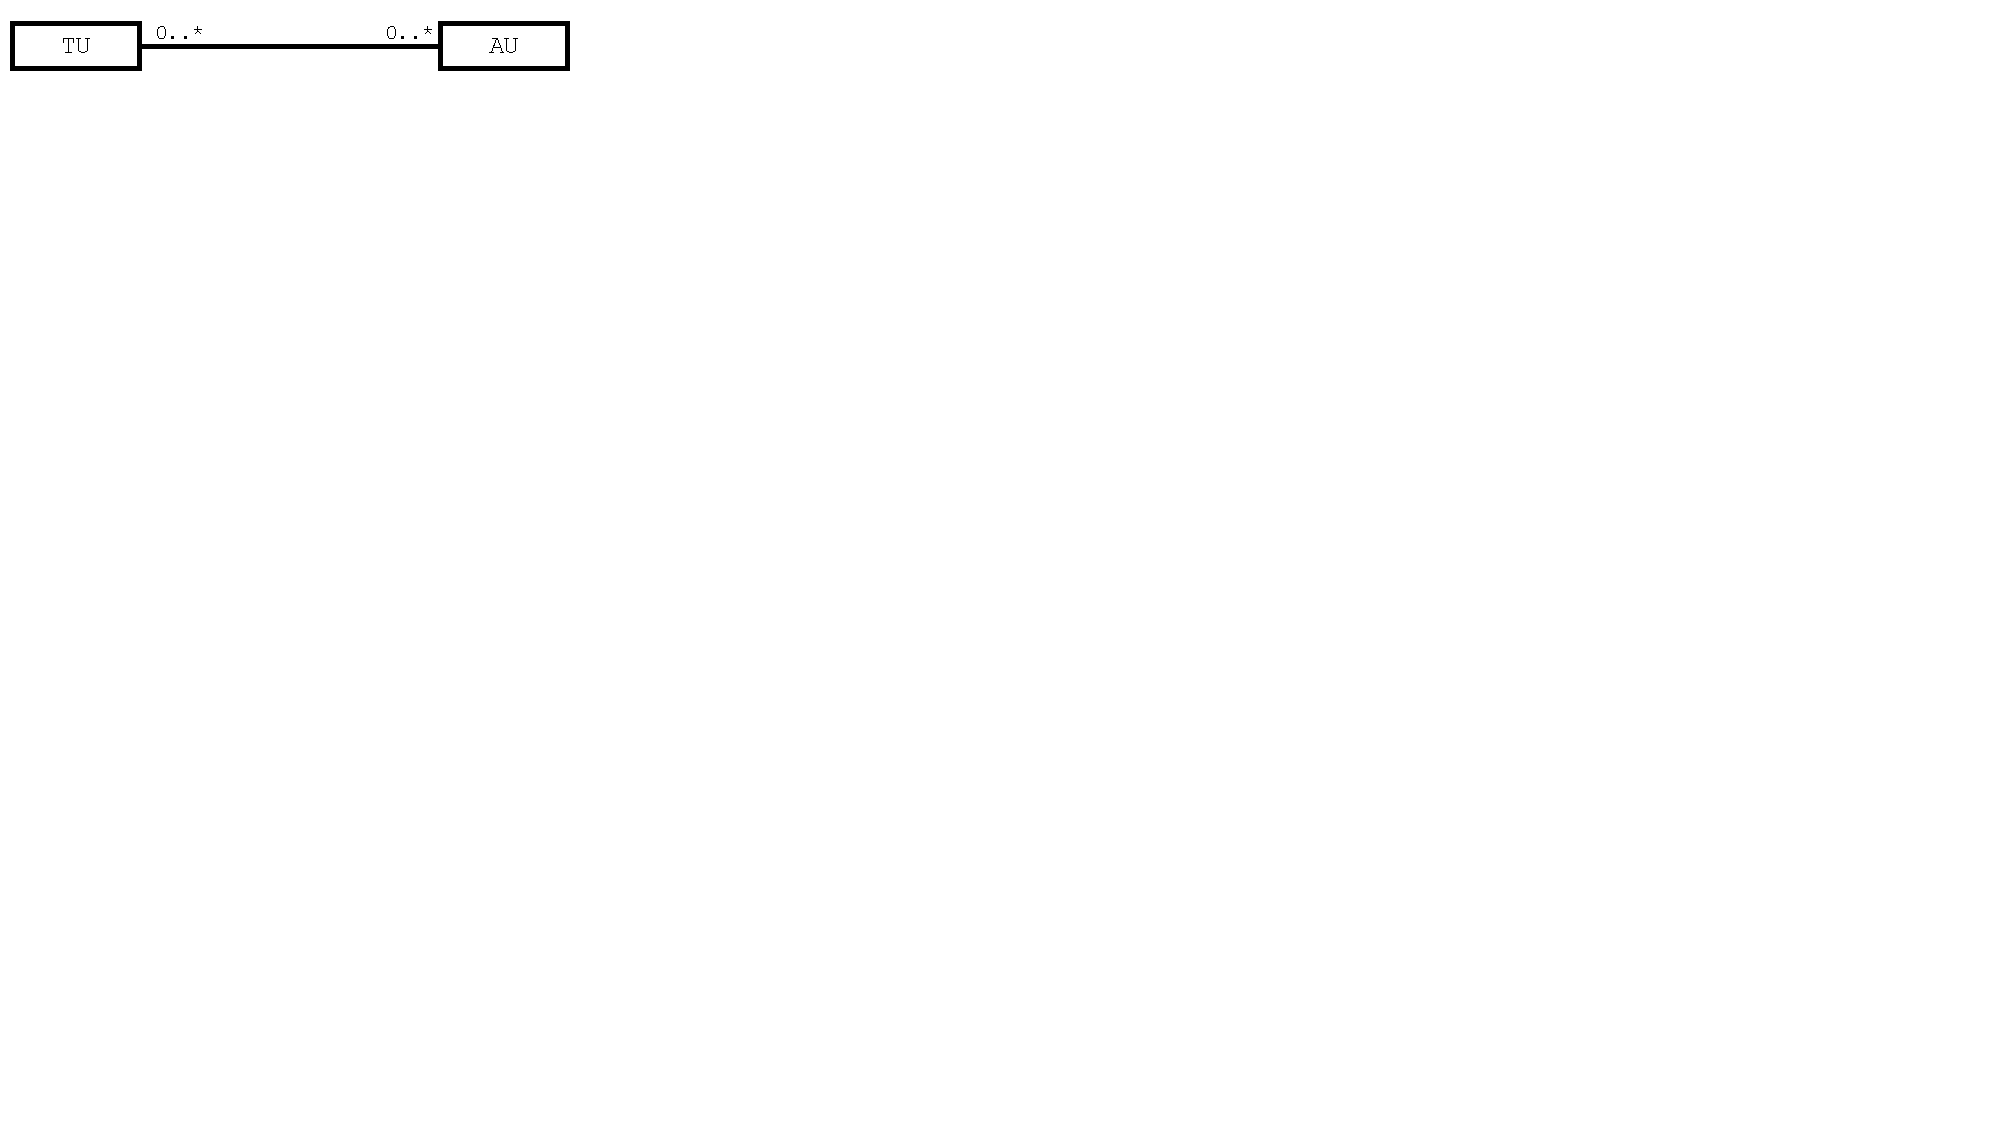
\includegraphics[width=\columnwidth,clip, trim=0cm 17.8cm 24.2cm 0.2cm]{TU-AU}%
   \caption{Relationship between Transformation (TU) and Animation (AU) Units for
   promoting multi-abstraction, and reuse.}%
   \label{fig:TU-AU}%
\end{figure}

To summarise our vision for enabling a systematic design of MA, we assume that a 
\DSL Engineer has already defined the core components, i.e. a metamodel capturing
the abstract syntax, one concrete syntax allowing to create, edit and manage 
conforming models, and a simulation that captures the \DSL's behaviour, specified
in an MTL that clearly defines TUs. The missing steps, and corresponding challenges,
for an MA Engineer, would be the following:

\begin{description}
   \item[C1.] How to explicitly model a Concrete Syntax, with sufficient details
   to support animation? Since MA basically consists of continuously updating the
   concrete syntax of a \DSL along its execution, an explicit representation of the
   concrete syntax that exposes the graphical features to the MA designer is 
   required.
   
   \item[C2.] How to explicitly model an MA compositionally, i.e. by creating an
   MA using basic components that are progressively composed in a fully-fledged
   animation representing the \DSL's behaviour visually? 
   
   \item[C3.] How to explicitly map TUs describing a \DSL's behaviour with the
   appropriate AU(s)? 
\end{description}
